\section{The Two Investigations}
\subsection{The Theoretical Investigation}
\subsubsection{Ansys Workbench}
\label{sec:ansysWorkbench}
The geometry and mesh preparation for the simulation was conducted using Ansys Workbench \parencite{noauthor_ansys_nodate}. The dimensions of the fluid domain are based on \ref{fig:fluidDomain} where l is the overall length of the bluff body.

\newlength\unitL
\setlength\unitL{0.2cm}

\begin{figure}[H]
	
	\begin{center}
		\begin{tikzpicture}[x=\unitL, y=\unitL, >=stealth, line width=1pt]
			
			% === Outer domain ===
			\draw (0,0) rectangle (63,50);
			
			% === Square obstacle ===
			\draw (22,24) rectangle (24,26);
			\draw[<->] (25, 24) -- (25, 26);
			\node at (27, 25) {$\ell$};  
			
			\draw[<->] (22, 23) -- (24, 23);
			\node at (23, 21) {$\ell$};  
			
			% === Velocity inlet arrows (spaced + farther from wall) ===
			\foreach \y in {12,20,28,36}
			\draw[->] (-5,\y) -- (-1,\y);  % stop at x=0.3 to add gap
			
			% === Velocity inlet label (more horizontal distance) ===
			\node[rotate=90] at (-7,25) {\large \textbf{Velocity Inlet}};
			
			% === Pressure outlet ===
			\draw[<->] (65.5,0) -- (65.5,50);
			\node[rotate=90] at (72,25) {\large \textbf{Pressure Outlet}};
			\node[rotate=90] at (68,25) {$50\,\ell$};
			
			% === Bottom dimensions (same horizontal alignment) ===
			\draw (23,0) -- (23,-0.8);  % tick at square center
			
			\draw[<->] (0,-3) -- (23,-3);  % from inlet to square center
			\node at (11.5,-5.1) {$23\,\ell$};
			
			\draw[<->] (23,-3) -- (63,-3); % from square center to outlet
			\node at (43,-5.1) {$40\,\ell$};
			
		\end{tikzpicture}
	\end{center}
	\caption{The fluid domain with dimensions. Inspired by \textcite{comflics_openfoam_2014}}
	\label{fig:fluidDomain}
\end{figure}

Given the computational limitations of the computer the simulation was conducted on, an overall length $\ell$ of $1\times{10}^{-3}$ meters was chosen, therefore giving each bluff body a characteristic length $L$ of $1\times{10}^{-3}$ meters. 

In order to create the mesh necessary for the simulation, the \textit{All Triangles Method} was utilized. A global unit size of $2.25\times{10}^{-3}$ meters was applied to the fluid domain to ensure a computationally inexpensive resolution in regions of negligible interest. Conversely, near the edge of the bluff body, a significantly smaller unit size of $2.0\times{10}^{-5}$ meters was used, constituting an accurate depiction of the interaction between the fluid flow and the bluff body \parencite{ansys_learning_best_2023}. Furthermore, eight inflation layers were employed in order to accurately capture the gradients associated with boundary layer formation at the edges of the bluff body \parencite{fluid_mechanics_101_cfd_2021}. Moreover, a body of influence (BOI) with a sizing of $2.0\times{10}^{-4}$ meters was used, positioned as shown in \ref{fig:fluidDomainWithBOI} below, in order to refine the mesh in the wake region, where the vortex shedding occurs, constituting for a more accurate simulation.  

\begin{figure}[H]
	
	\begin{center}
		\begin{tikzpicture}[x=\unitL, y=\unitL, >=stealth, line width=1pt]
			
			% === Outer domain ===
			\draw (0,0) rectangle (63,50);
			
			% === BOI rectangle ===
			\draw[dashed] (15,17) rectangle (63,33);  % Body of Influence
			\node[anchor=south west] at (36,33) {\textbf{BOI}};
			
			% === Square obstacle ===
			\draw (22,24) rectangle (24,26);
			\draw[<->] (25, 24) -- (25, 26);
			\node at (27, 25) {$\ell$};  
			
			\draw[<->] (22, 23) -- (24, 23);
			\node at (23, 21) {$\ell$};  
			
			% === Velocity inlet arrows (spaced + farther from wall) ===
			\foreach \y in {12,20,28,36}
			\draw[->] (-5,\y) -- (-1,\y);  % stop at x=0.3 to add gap
			
			% === Velocity inlet label (more horizontal distance) ===
			\node[rotate=90] at (-7,25) {\large \textbf{Velocity Inlet}};
			
			% === Pressure outlet ===
			\draw[<->] (65.5,0) -- (65.5,50);
			\node[rotate=90] at (72,25) {\large \textbf{Pressure Outlet}};
			\node[rotate=90] at (68,25) {$50\,\ell$};
			
			% === Bottom dimensions (same horizontal alignment) ===
			\draw (23,0) -- (23,-0.8);  % tick at square center
			
			\draw[<->] (0,-3) -- (23,-3);  % from inlet to square center
			\node at (11.5,-5.1) {$23\,\ell$};
			
			\draw[<->] (23,-3) -- (63,-3); % from square center to outlet
			\node at (43,-5.1) {$40\,\ell$};
			
		\end{tikzpicture}
	\end{center}
	\caption{The fluid domain with dimensions. Inspired by \textcite{comflics_openfoam_2014}}
	\label{fig:fluidDomainWithBOI}
\end{figure}

\subsubsection{The OpenFoam Simulation}
The theoretical part of this EE is conducted using the open-source CFD software package OpenFOAM \parencite{noauthor_openfoam_2024}. Among the numerous solvers OpenFOAM provides, pimpleFOAM is a transient, pressure-based solver for incompressible, single-phase, also referred to as isothermal, flows \. It combines the algorithms used in the pisoFOAM and simpleFOAM solvers, enabling robust handling of transient simulations with larger time steps, allowing for improved computational performance, hence why the solver was chosen. Moreover, its ability to model both laminar and turbulent flow ensures flow conditions are accurately reflected and given that the fluctuations of lift force are sinusoidal, one can verify the flow is laminar. Utilizing reporting functions, one can extract the lift coefficient $C_{L}$, which shows the fluctuations in the lift force acting on the bluff body.
\subsubsection{Simulation Settings}
To adhere to the scope of this essay, the simulation setup is adapted from a case study provided in the Udemy course OpenFOAM for Absolute Beginners by \textcite{jayaraj2024openfoam}. The tutorial case \textit{3vortexShedding}, discussed in lecture eight, serves as a structural template and has been modified to align with the specific requirements of this investigation.

\begin{figure}[H]
	\centering
	\begin{forest}
		for tree={
			font=\ttfamily,
			grow=east,
			child anchor=west,
			parent anchor=east,
			anchor=west,
			edge={draw,-stealth},
			inner sep=2pt,
			l sep=50pt,
			s sep=20pt
		}
		[case/
		[0/
		[\textcolor{blue}{U}]
		[p]
		[nuTilda]
		[nut]
		]
		[constant/
		[turbulenceProperties]
		[\textcolor{blue}{transportProperties}]
		[g]
		[\textcolor{green}{polyMesh/}
		[\textcolor{green}{pointZones}]
		[\textcolor{green}{points}]
		[\textcolor{green}{owner}]
		[\textcolor{green}{neighbor}]
		[\textcolor{green}{faceZones}]
		[\textcolor{green}{faces}]
		[\textcolor{green}{cellZones}]
		[\textcolor{green}{boundary}]
		]
		]
		[system/
		[fvSolution]
		[fvSchemes]
		[\textcolor{green}{forceCoeffs}]
		[\textcolor{blue}{decomposeParDict}]
		[\textcolor{blue}{controlDict}]
		]
		[\textcolor{blue}{para.foam}]
		[\textcolor{blue}{mesh.msh}]
		]
	\end{forest}
	\caption{Overview of the simulation directory structure. Modified files are highlighted blue. Created files and folders are highlighted green }
\end{figure}


\begin{table}[H]
	\centering
	\renewcommand{\arraystretch}{1.3}
	\makebox[\linewidth][c]{
		\begin{tabularx}{1.2\textwidth}{|p{3cm}|p{3.3cm}|p{2.8cm}|p{3cm}|X|}
			\hline
			\textbf{File} & \textbf{Parameter} & \textbf{Original} & \textbf{Modified} & \textbf{Justification} \\
			\hline
			\verb*|mesh.msh|, \verb*|para.foam|, 
			\begin{tabular}[t]{@{}l@{}}
				\verb|polyMesh/|\\[-0.3em]
				\small\hspace{1.5em}\verb|boundary| \\[-0.3em]
				\small\hspace{1.5em}\verb|cellZones| \\[-0.3em]
				\small\hspace{1.5em}\verb|faces| \\[-0.3em]
				\small\hspace{1.5em}\verb|faceZones| \\[-0.3em]
				\small\hspace{1.5em}\verb|neighbor| \\[-0.3em]
				\small\hspace{1.5em}\verb|owner| \\[-0.3em]
				\small\hspace{1.5em}\verb|points| \\[-0.3em]
				\small\hspace{1.5em}\verb|pointsZones|
			\end{tabular} 
			
			& \textemdash & \verb*|mesh.msh| defines, \verb*|polyMesh/| contains and \verb*|para.foam| visualizes the mesh of fluid domain of tutorial case & \verb*|mesh.msh| defines, \verb*|polyMesh/| contains and \verb*|para.foam| visualizes the mesh of fluid domain with dimensions given in \Cref{sec:ansysWorkbench} & The fluid domain has been adjusted to conform with the computational limits discussed in \Cref{sec:ansysWorkbench}, while achieving the Reynolds number required for this investigation\\
			\hline
			\verb*|controlDict| & \verb*|deltaT| & 0.0002 & 0.00001 &
			Decreased in order to achieve a greater accuracy \parencite[289]{versteeg2007} while ensuring numerical stability \parencite{caminha_cfl_2017}. 
			\\
			
			\rule{0pt}{5ex} & \verb*|functions| & \verb*|none| &
			\begin{tabular}[t]{@{}l@{}}
				\verb|#include| \\[-0.3em]
				\verb*|"forceCoeffs"|
			\end{tabular} &
			Reporting function defined in \verb*|forceCoeffs| included in order to extract the lift coefficient $C_L$ \parencite{codeynamics_prism_2024}
			\\ 
			
			\rule{0pt}{5ex} & {\small\verb*|adjustTimeStep|} & \verb*|yes| & \verb*|no| &
			Removed as the simulation demonstrated stable behavior with the adjusted \verb*|deltaT| \parencite{jayaraj2024openfoam}
			\\ 
			
			\hline
			
			{\footnotesize\verb*|decomposeParDict|} & {\footnotesize\verb*|numberOfSubdomains|} & 8 & 6 & The simulations are performed on a system with \verb*|6| processing cores \parencite{jayaraj2024openfoam} \\
			\hline
			
			\verb*|forceCoeffs| & \textemdash & \textemdash & Created a reporting function which outputs the variation of the lift coefficient $C_L$ throughout the simulation & Lift coefficient $C_L$ needed for subsequent calculation of vortex shedding frequency $f$\\
			\hline
			
			
		\end{tabularx}
	}
	\caption{Overview of the changes made to the simulation template.}
	\label{tab:simulation_change1}
\end{table}

\begin{table}[H]
	\centering
	\renewcommand{\arraystretch}{1.3}
	\makebox[\linewidth][c]{
		\begin{tabularx}{1.2\textwidth}{|p{3cm}|p{3.3cm}|p{2.8cm}|p{3cm}|X|}
			\hline
			\textbf{File} & \textbf{Parameter} & \textbf{Original} & \textbf{Modified} & \textbf{Justification} \\
			\hline
			
			{\scriptsize\verb*|transportProperties|} & \verb*|nu| & $1\times 10^{5}$ & $1\times 10^{6}$ & The kinematic viscosity of water at 20°C is approximately $1\times 10^{6} \, m^2\,s^{-1}$ \parencite{noauthor_water_nodate}\\
			\hline
			\verb*|U|& \texttt{inlet value} \newline \texttt{(x, y, z)} & x = 10 & x = 0.1 & Adapted in order to achieve the target Reynolds number of 100 using Equation~\eqref{eq:reynoldsNumber} where $L=1\times 10^{-3} \, m$ and $\nu = 1\times10^{-6} \, m^2\,s^{-1}$ \\
			\hline
		\end{tabularx}
	}
	\caption*{Table 1 (continued): Overview of the changes made to the simulation template.}
	\label{tab:simulation_changes2}
	
\end{table}



\subsection{The Practical Investigation}
Inspired by the flow tank built by Harvard University’s Science Demonstrations Center \parencite{noauthor_vortex_nodate}, the practical part of this EE will be conducted in a self-built flow tank, utilizing a water pump and a separation wall to create flow over a horizontal plate \textemdash\ the water pump moves the water from one side of the separation wall to the other. A second separation wall which fails to reach the bottom of the tank forces the water flowing over the horizontal wall towards the pump. The regulation valve is used to modulate the flow velocity while the sponge diffuser decreases the flow velocity and ensures a uniform distribution of flow. Both a lamp and the addition of potassium permanganate crystals in front of the shape are used in order to better visualize the water flow. The thermal insulation foam ensures watertightness between the aquarium wall and the inside components.

\begin{figure}[H]
	\centering
	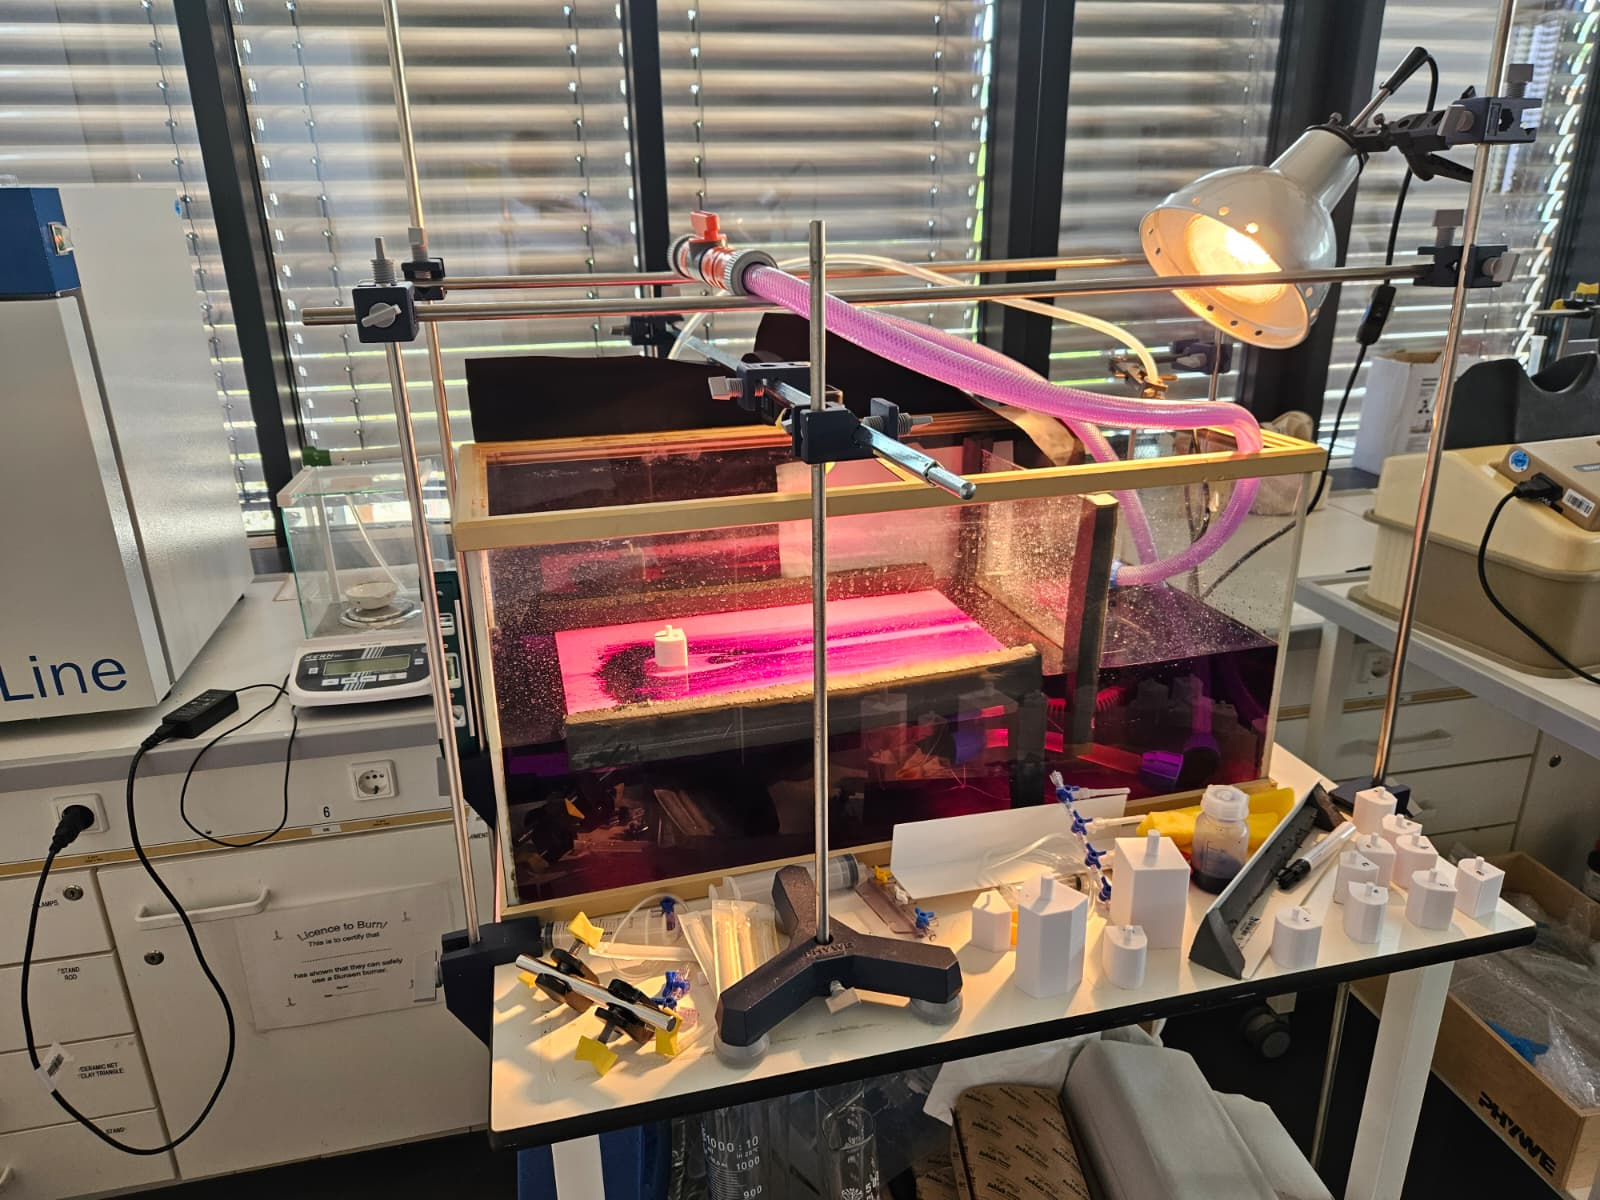
\includegraphics[width=\textwidth]{images/overallSetup.jpg}
	\caption{The setup for the practical investigation}
	\label{fig:overallSetup}
\end{figure}

\begin{figure}[H]
	
	\begin{center}
		\begin{tikzpicture}[x=\unitL, y=\unitL, >=stealth, line width=1pt]
			
		\end{tikzpicture}
	\end{center}
	\caption{The fluid domain with dimensions. Inspired by \textcite{comflics_openfoam_2014}}
	\label{fig:practicalSetup}
\end{figure}

The bluff bodies were 3D printed with an overall length $\ell$ of $0.02$ meters \textemdash\ as described in \Cref{sec:bluffBody} \textemdash\ giving each shape a characteristic length $L$ of $0.02$ meters and a height of $0.04$ meters. Reference marks on the horizontal plate ensure the shape is positioned in the same position each trial. A GoPro is mounted parallel to the horizontal plate, ensuring a continuous recording of the entire horizontal plate.

\begin{figure}[H]
	\centering
	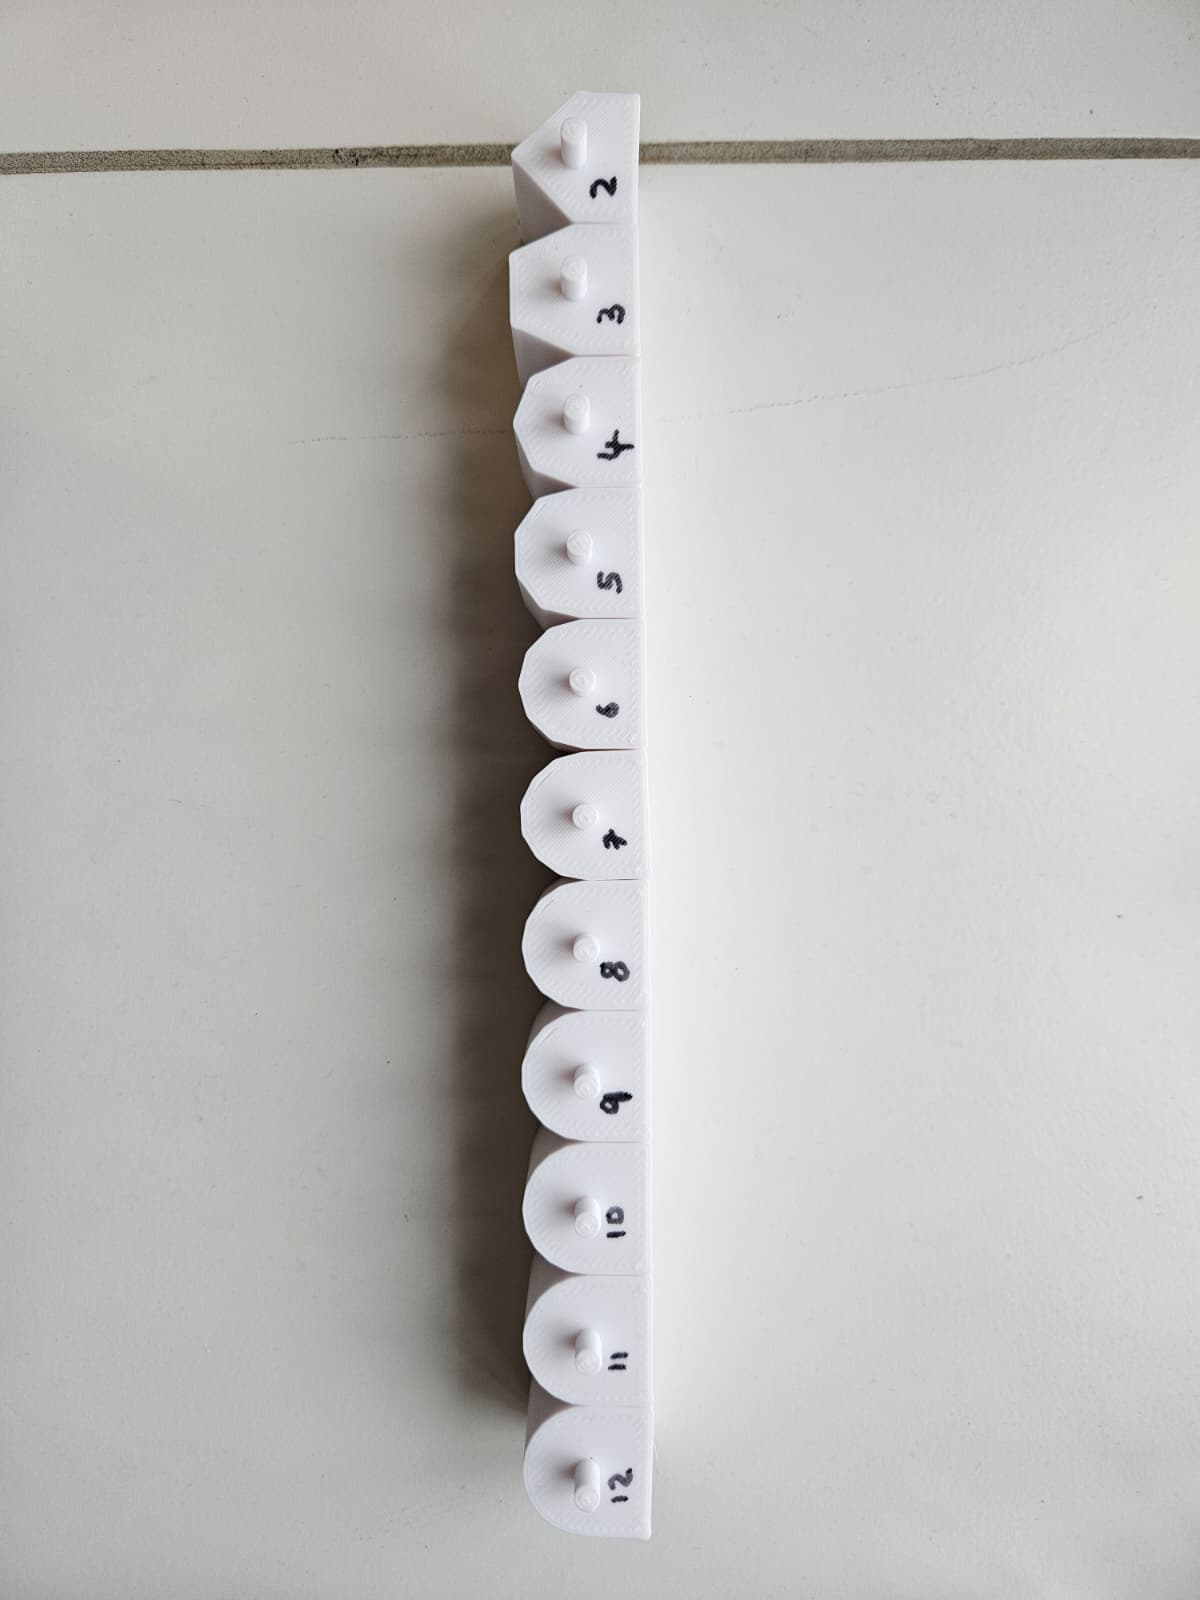
\includegraphics[width=\textwidth]{images/shapes.jpg}
	\caption{The 3D-printed bluff bodies}
	\label{fig:shapes}
\end{figure}

\begin{figure}[H]
	\centering
	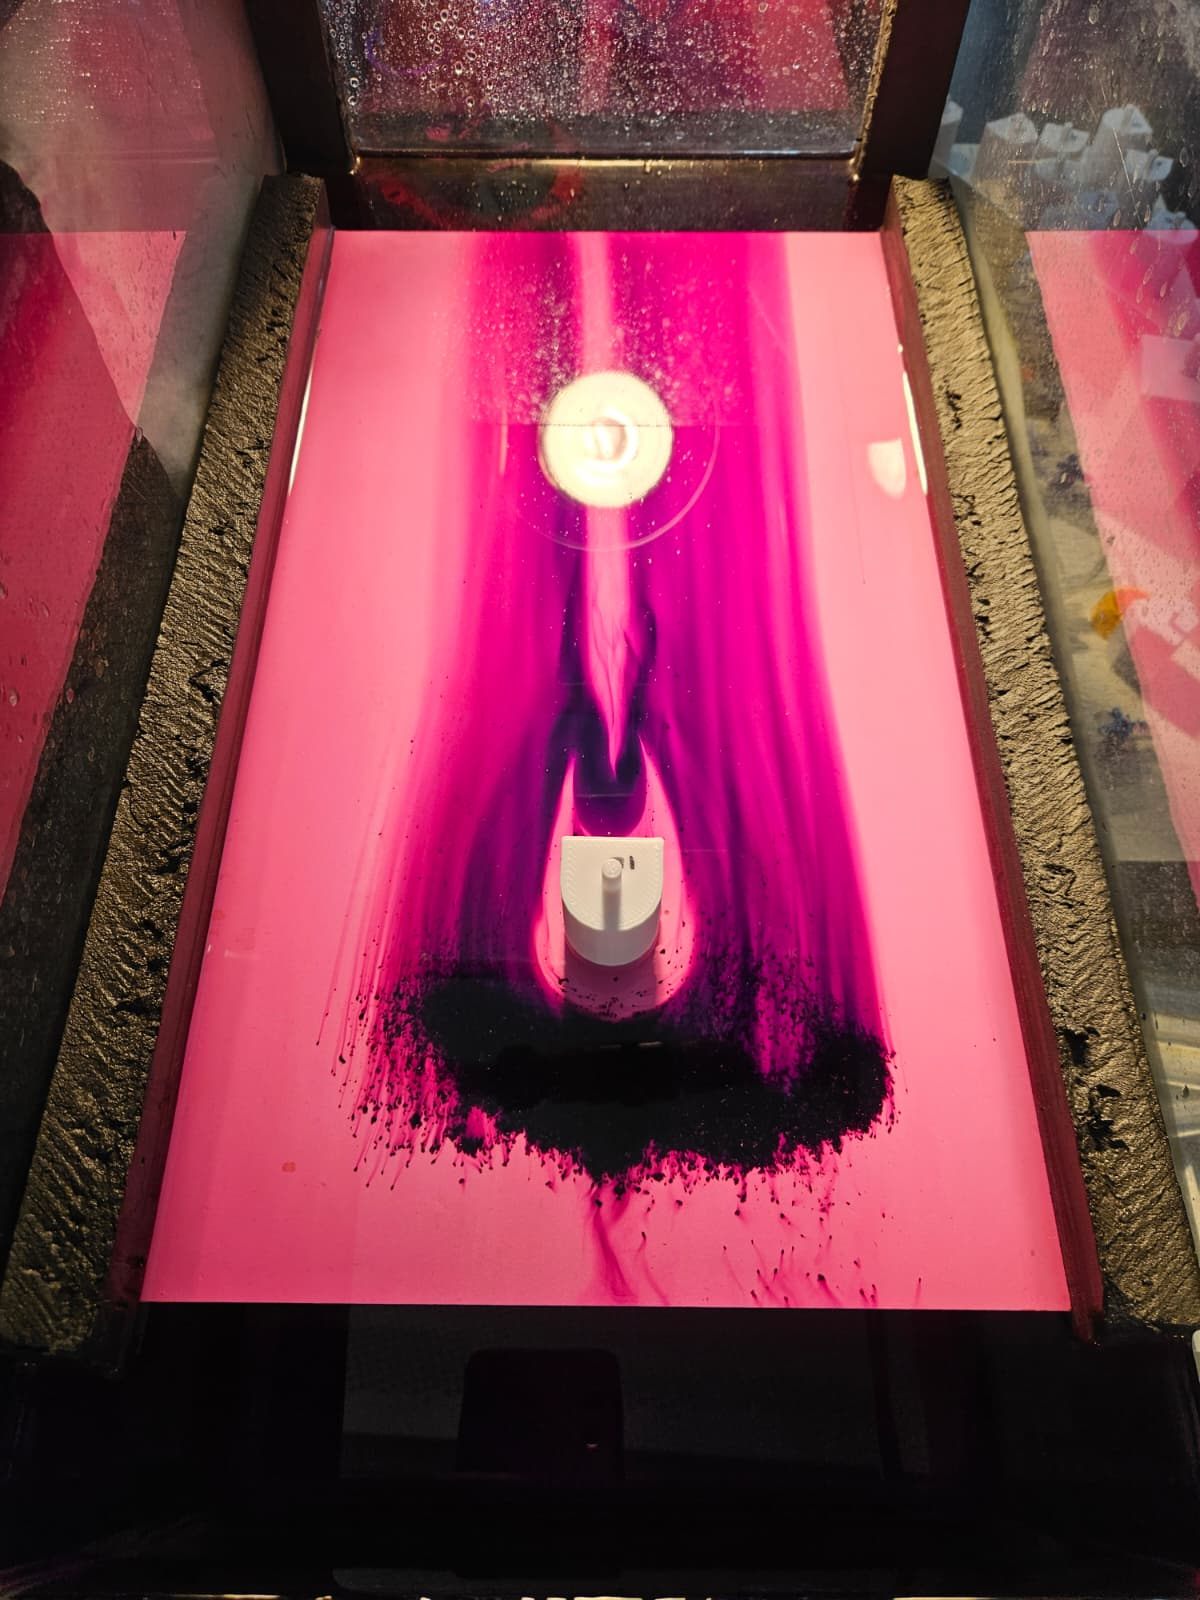
\includegraphics[width=\textwidth]{images/shapeInTank.jpg}
	\caption{A bluff body positioned in the flow tank with potassium permanganate crystals spread in front of it}
	\label{fig:shapeInTank}
\end{figure}

\subsection{Determining the vortex shedding frequency}
The inverse relationship given by Equation \eqref{eq:fAndT} in section \Cref{sec:fAndT} will be used to determine the vortex shedding frequency. By measuring the time interval between the formation of two consecutive vertices on one side of the bluff body, one can find the time period and therefore the frequency of vortex shedding. To obtain an accurate vortex shedding frequency, the determination of the time period was done multiple times and was only done in the steady-state phase, when the velocity and pressure at any given point in the system remain constant \parencite{noauthor_steady_nodate}, omitting the initial transient phase, when the velocity and pressure vary over time \parencite{noauthor_transient_nodate}. A Fast Fourier Transform approach was not chosen due to the lack of sufficient run time during the trials on either investigation \parencites[10--11]{shi2025vortex}[12]{xu_experimental_2025}.